\documentclass[12pt]{report}

\newcommand{\titletext}{Semilinaire spectraalanalyse}

\usepackage[dutch]{babel}
\usepackage[nobottomtitles]{titlesec}
\usepackage[bottom]{footmisc}
\usepackage{graphicx}
\usepackage{titleps}
\usepackage{amssymb}
\usepackage{amsmath}
\usepackage{amsthm}
\usepackage{graphicx}
\usepackage{verbatim}
\usepackage{titling}
\usepackage[toc,page]{appendix}
\usepackage{bm}
\usepackage{wrapfig}
\usepackage{subcaption}

\usepackage{fancyhdr}

\pagestyle{fancy}

\renewcommand{\chaptermark}[1]{\markboth{#1}{}}
\renewcommand{\sectionmark}[1]{\markright{#1}}
\fancyhf{}
\fancypagestyle{plain}{%
  \fancyhf{}%
	\rfoot{\fancyplain{}{\nouppercase{\thepage}}}
	\lfoot{\fancyplain{}{Thorvald Dox}}
  \renewcommand{\headrulewidth}{0pt}% Line at the header invisible
  \renewcommand{\footrulewidth}{0.4pt}% Line at the footer visible
}
\lhead{\fancyplain{}{\titletext}}
\rhead{\fancyplain{}{\nouppercase{\leftmark}}}
\rfoot{\fancyplain{}{\nouppercase{\thepage}}}
\lfoot{\fancyplain{}{Thorvald Dox}}
\renewcommand{\footrulewidth}{0.4pt}

\fancyhfoffset[E,O]{0pt}
\date{}
  
\usepackage[margin=1in]{geometry}
\usepackage{float}



\usepackage[super,square,sort]{natbib}
\usepackage{bibentry}
\nobibliography*

%\newcommand{\footcite}[1]{\cite{#1}\let\thefootnote\relax \footnote{\cite{#1} \bibentry{#1}} }
\def\signed #1{{\leavevmode\unskip\nobreak\hfil\penalty50\hskip2em
  \hbox{}\nobreak\hfil(#1)%
  \parfillskip=0pt \finalhyphendemerits=0 \endgraf}}
\newcommand{\rulesep}{\unskip\ \vrule height -1ex\ }

\DeclareMathOperator*{\Odot}{\bigodot}
\allowdisplaybreaks

%\title{Semi-lineair Multiple Endmember mixture spectrum analysis}
\title{\titletext}
\author{Thorvald Dox}

\begin{document}
\begin{titlepage}

\newcommand{\HRule}{\rule{\linewidth}{0.5mm}} % Defines a new command for the horizontal lines, change thickness here

\center % Center everything on the page
 
%----------------------------------------------------------------------------------------
%	HEADING SECTIONS
%----------------------------------------------------------------------------------------

\textsc{\LARGE Universiteit Antwerpen}\\[1.5cm] % Name of your university/college
\textsc{\Large Fysica}\\[0.5cm] % Major heading such as course name
\textsc{\large Masterproef}\\[0.5cm] % Minor heading such as course title

%----------------------------------------------------------------------------------------
%	TITLE SECTION
%----------------------------------------------------------------------------------------

\HRule \\[0.4cm]
{ \Large \bfseries \thetitle}\\[0.4cm] % Title of your document
\HRule \\[1.5cm]
 
%----------------------------------------------------------------------------------------
%	AUTHOR SECTION
%----------------------------------------------------------------------------------------

\begin{minipage}{0.4\textwidth}
\begin{flushleft} \large
\emph{Auteur:}\\
\theauthor % Your name
~\\
~\\
~\\
\end{flushleft}
\end{minipage}
~
\begin{minipage}{0.4\textwidth}
\begin{flushright} \large
\emph{Promotor:} \\
Paul {Scheunders} \\ % Supervisor's Name
\emph{Copromotor:} \\
Rob {Heylen} % Supervisor's Name
\end{flushright}
\end{minipage}\\[5cm]

% If you don't want a supervisor, uncomment the two lines below and remove the section above
%\Large \emph{Author:}\\
%John \textsc{Smith}\\[3cm] % Your name

%----------------------------------------------------------------------------------------
%	DATE SECTION
%----------------------------------------------------------------------------------------

%{\large \today}\\[3cm] % Date, change the \today to a set date if you want to be precise

%----------------------------------------------------------------------------------------
%	LOGO SECTION
%----------------------------------------------------------------------------------------

%
\includegraphics[height=4cm]{remote.png}

\includegraphics[height=4cm]{download.jpg}
\hspace{5 cm}

\includegraphics[height=4cm]{vlabsym.png}
 \\[1cm] % Include a department/university logo - this will require the graphicx package

 
%----------------------------------------------------------------------------------------

\vfill % Fill the rest of the page with whitespace

\end{titlepage}
\tableofcontents


\newpage
\chapter*{Abstract}
\addcontentsline{toc}{chapter}{Abstract (english)}


\newpage
\chapter*{Abstract}
\addcontentsline{toc}{chapter}{Abstract (Nederlands)}



\newpage
\chapter*{Structuur van deze thesis}
\addcontentsline{toc}{chapter}{Structuur van deze thesis}

De inleiding legt uit wat aardopservatie is, welke concepten hiervoor nodig zijn en een aantal toepassingen hiervoor. Dit hoofdstuk is vooral gebaseerd op \textit{Fundamentals of remote sensing\cite{fun}}.

Het eerste hoofdstuk gaat over ontmengen. Hier wordt wordt het concept ontmengen uitgelegd, en een voorbeeld gegeven hiervan, namelijk lineair ontmengen. 

In het volgende hoofdstuk worden drie bestaande methodes uitgelegd. Het eerste deel gaat over het multilinair model, en is gebaseerd op \textit{A multilinear mixing model for nonlinear spectral unmixing}\cite{mlinmix}. De volgende delen gaan over selectiemethoden. Dit zijn methoden ontwikkeld om om te gaan met endmembervariabiliteit. Deze methoden staan beschreven in \textit{Hyperspectral unmixing with endmember variability via alternating angle minimization}\cite{mesma}. Deze methoden zijn volledig gekend in de literatuur maar voor deze thesis zijn deze methoden opnieuw berekend en ge\"implementeert. 

Het derde hoofdstuk beschrijft twee nieuwe methoden, gebaseerd op de methoden beschreven in het vorige hoofdstuk, Ook wordt er van de eerste methode een numeriek bewijs geleverd dat deze goede resultaten geeft door middel van monte-carlo simulaties. 

In het laatste hoofdstuk worden al deze methoden, en een aantal varianten hierop vergeleken aan de hand van een experimentele dataset: de Alina dataset\cite{Alina} en wordt besproken welke methodes en varienten het beste zijn in welke situaties. 
\newpage
\chapter*{Inleiding}
\addcontentsline{toc}{chapter}{Inleiding}

\begin{quotation}
Aardobservatie is de wetenschap van het bepalen van informatie over het aardoppervlak vanop een afstand. Dit wordt gedaan door het meten en vastleggen van gereflecteerde of uitgezonden energie en het verwerken, analyseren en toepassen van deze informatie.
\signed{\textit{Fundamentals of remote sensing\cite{fun} p5}}
\end{quotation}

\begin{wrapfigure}{R}{0.4\textwidth}
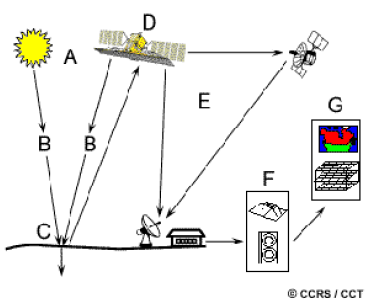
\includegraphics[width=0.4\textwidth]{rs.PNG}
\caption{Aardopservatie \label{fig:rs} Deze afbeelding komt uit \textit{Fundamentals of remote sensing\cite{fun}}}
\end{wrapfigure}


Het gedetai\"eerde process verloopt zoals hierna beschreven\cite{fun}, en is te zien in figuur \ref{fig:rs} .

Een lichtstraal ontstaat aan een zo genaamde lichtbron\footnote{In het geval dat men geintereseert is in het termisch infrarood spectrum, is er geen lichtbron nodig aangezien materialen op kamertemperatuur van nature dit soort licht uitstralen, ten gevolge van black body radiation.}. In de meeste gevallen is deze lichtbron de zon. Deze lichtstraal reist door de ruimte en door de atmosfeer, tot deze contact maakt men het materiaal, en hierop een of meerdere keren reflecteert. Daarna reist deze lichtstraal opnieuw door de atmosfeer tot deze contact maakt met een camera op een sateliet. De eigenschappen van deze lichtstraal worden be\"invloed door elk van deze processen.





Elke lichtstraal is een golf in het elektromagnetische spectrum. Deze golf wordt enerzijds bepaald door zijn golflengte, wat de lengte is tussen twee opeenvolgende maxima van de golf, zoals afgebeeld in figuur \ref{fig:golflengte}. Anderzijds wordt de golf bepaald door de intensiteit, wat de grootte is van de piek van elke golf. Soms wordt de frequentie van de golf gebruikt om deze te karakteriseren, maar die kan bepaald worden uit de golflengte en de snelheid van het licht. In werkelijkheid is een lichtstraal niet een golf, maar een combinatie van verschillende golven met elk hun golflengte en intensiteit. De bijbehorende intensiteit bij elke golflengte wordt het spectrum genoemd.




Gewone beelden van een camera bevatten drie kleuren, elke passend bij een specifieke golflengte. De keuze voor deze drie kleuren, namelijk rood, groen en blauw, is een gevolg van de beperkingen van het menselijk oog. Dit zijn namelijk de kleuren dat een mens kan waarnemen. Om dit beeld digitaal te representeren, moet het beeld opgedeeld worden in kleine, even grootte, vierkante elementen, genaamd pixels. Elk van deze pixels bevat voor elke kleur een waarde, die de intensiteit van deze kleur in dit vierkant weergeeft. Hyperspectrale cameras werken in essentie op dezelfde manier, alleen detecteert deze camera niet alleen de hoeveelheid rood, groen en blauw, maar detecteert deze een groot aantal banden. Doordat deze banden meer informatie bevatten dan de banden van een gewone camera, kan hier meer informatie uit gehaald worden. Omdat de zon vooral licht uitzend in het infrarood, zichtbaar licht en ultraviolet worden er vooral banden gebruikt in dit spectrum, zoals te zien in figuur \ref{fig:specs}.  


\begin{figure}
\center
\begin{subfigure}[b]{0.3\textwidth}
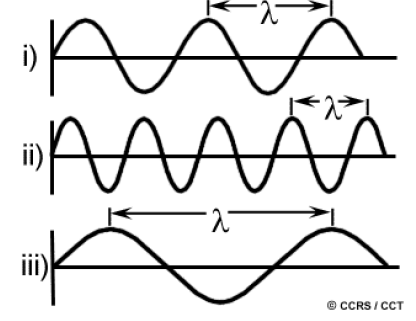
\includegraphics[width=\textwidth]{golflengte.PNG}
\caption{Golven met verschillende golflengten \label{fig:golflengte}}
\end{subfigure} \rulesep
\begin{subfigure}[b]{0.2\textwidth}
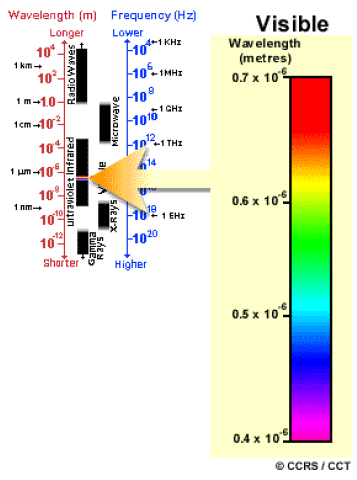
\includegraphics[width=\textwidth]{spec.PNG}
\caption{Het electromagnetische spectrum. \label{fig:spec}}
\end{subfigure}\rulesep
\begin{subfigure}[b]{0.4\textwidth}
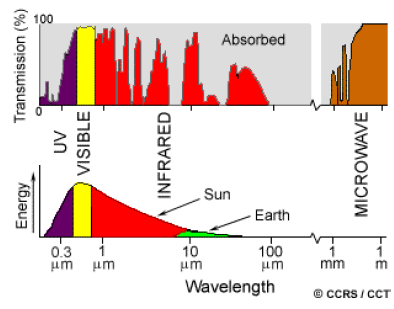
\includegraphics[width=\textwidth]{spec2.PNG}
\caption{Het spectrum van de zon. \label{fig:specs}}
\end{subfigure}
\caption{electromagnetische golven. Deze afbeeldingen komen uit \textit{Fundamentals of remote sensing\cite{fun}}}
\end{figure}


Het doel van spectrale analyse is het bepalen van de hoeveelheden van elk materiaal in een specifieke pixel, gegeven het spectrum van deze pixel. Verschillende methoden hiervoor worden beschreven in deze thesis. 


\section{toepassingen}


Een veelgebruikte toepassing van aardopservatie is het in kaart brengen van landbouwgewassen\cite{fun}. Men kan niet alleen het soort gewas op een akker in kaart brengen, maar ook onder andere de gezondheid en verwachte oogst van verschillende gewassen. Deze informatie is nuttig voor de landbouwers zelf, omdat deze aan de hand van de data kunnen bepalen welke gewassen het beste groeien op welke plaats en wanneer er het best gezaaid of geoogst wordt. Ook is dit nuttig voor overheden en verzekeraars, omdat deze kunnen nagaan welke planten er geplant worden, kunnen voorspellen wat de oogst gaat zijn en kunnen bepalen wat de schade is na een droogte of storm. In het verleden werd het in kaart brengen van gewassen gedaan door steekproeven te nemen met de hand vanop de grond, maar aardopservatie is nauwkeuriger, goedkoper en kan eenvoudiger gestandaardiseerd worden. 

Een andere toepassing is geologie. Men kan het soort gesteente van het aardoppervlak in kaart brengen, maar ook de formatie en zelfs gesteentes onder het aardoppervlak. Een van de voor de hand liggende toepassingen hiervan is de mijnbouw, maar dit kan ook gebruikt worden voor het voorspellen van aardbevingen, aardverschuivingen en vulkanisme. Daarom kan dit gebruikt worden voor het plannen van wegen, gebouwen en andere structuren. Meestal word deze data gebruikt in combinatie met data verzameld op de grond, namelijk radarbeelden. 

  
\begin{figure}
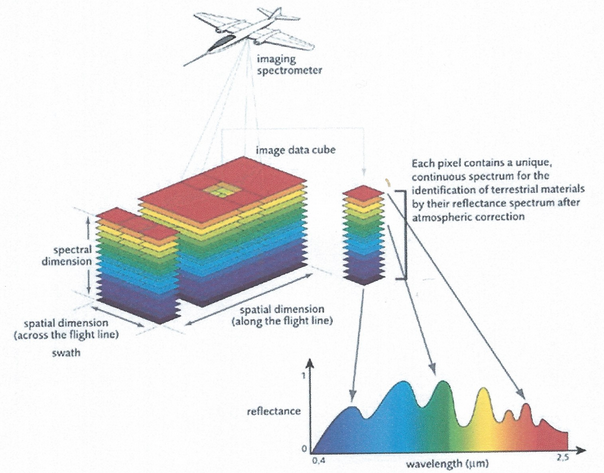
\includegraphics[width=\textwidth]{hyp.PNG}
\caption{Opbouw van een hyperspectraal beeld. Deze afbeelding komt uit \textit{Fundamentals of remote sensing\cite{fun}}}
\end{figure}

\chapter{ontmengen}



%Het doel van spectrale anaylise is om uit deze hyperspectrale beelden het bepalen welke materialen zich op een specifieke pixel bevinden. Hoewel het belangrijkste toepassing hiervan de aardopservatie is, kan dit evidenterwijs ook gebruikt worden om materialen te analyseren in een laboratorium of voor bijvoorbeeld kwaliteitscontrole in de industrie.


Een pixel in een hyperspectraal beeld bevat meerdere materialen. Een van de belangrijkste oorzaken is het gevolg van de beperkte resolutie van de camera. Echter, de hoeveelheid licht dat op de camera valt is beperkt, en moet verdeelt worden over de verschillende pixels en de verschillende banden. Dit betekend dat wanneer de pixels te klein worden, elke pixel te weinig licht krijgt en de signaal ruis verhouding te laag wordt. En aangezien de licht bestaat uit fotonen, is er een limiet van de gevoeligheid van de camera, en is de enige methode om de gevoeligheid te verhogen een langere belichtstijd. Dit zorgt vor een vergrotting van de ruis en is niet haalbaar voor een satelliet in een baan rond de aarde. Maar zelfs als het praktisch haalbaar was om de resolutie kleiner te maken, ligt het probleem vooral in de fractalische eigenschappen van veel objecten. Neem nu bijvoorbeeld een bos. Als we een zeer grove resolutie gebruiken, vallen er verschillende soorten bomen in een enkele pixel. Als de pixels kleiner worden, kunnen bomen al van elkaar onderscheiden worden, maar de takken van verschillende bomen nog niet. Zelfs als we enkel een blad beschouwen zijn er nog verschillende materialen, aangezien de nerven van het blad een ander materiaal hebben dan de bladmoes. Een ander voorbeeld zijn mineralen. Een gesteente bevat verschillende mineralen, maar om deze van elkaar te kunnen onderscheiden moet de pixelgrootte al op microscopisch niveau zijn. 

Hierom is het van belang om een spectra van een pixel, dat een combinatie is van de spectra van de verschillende materialen in deze pixel, te kunnen ``ontmengen''. Hierbij zijn we specifiek ge\"intereseerd in de abundantie van elk materiaal: een getal dat het gedeelte van de lichtstralen dat afkomstig is van dat specifiek materiaal weergeeft. Aangezien dit een goede maat is voor de aanwezige hoeveelheid van een bepaald materiaal in een pixel, is dit de belangrijkste parameter waarin we ge\"intereseerd zijn.


\section{spectrale analyse}


Het spectra van licht kan beschreven worden als een wiskunde functie die een frequentie omzet in een intensiteit. In werkelijkheid bevat een hyperspectraal beeld niet de volledige functie, maar bevat deze tweehonderd waarden in deze functie, de zogenoemde banden. Dit matlab\citep{MATLAB} zal dit worden opgeslagen als een driedimensinale tensor, waarbij de verschillende assen de x positie, y positie en band van de pixel weergeven. In deze thesis zijn we niet geintereseerd in  interpixel-interacties, wat betekend dat het materiaal in een pixel geen invloed heeft op het spectrum van andere pixels. Daardoor kan de drie-dimentionale matrix worden omgezet in een matrix, waar de rijen de verschillende pixels zijn en de colommen de de banden.  

Endmembers zijn de spectra van de verschillende materialen waarin het beeld wordt ontmengd. Echter, om een goede theroie te construeren om deze spectra te ontmengen, moet eerst een model ontwikkeld worden om deze spectra te ontmengen. De meest voor de hand liggende methode is de linaire methode, waar het spectrum van elke endmember wordt vermenigvuldigd met de abundantie, en dan worden alle spectra opgeteld. 
%\begin{itemize}
%\item spectra als functies (eigenschappen van licht)
%\item spectra als vector (endmembers) $\rightarrow$ matlab implementatie
%\item mengen van endmembers (abundancies)
%\end{itemize}

\subsection{reflectie}

%Wanneer een lichtstraal invalt op een materiaal reflecteert deze een gedeelte van dit licht. Het nieuwe spectrum van het gereflecteerde licht kan bepaald worden aan de hand van de eigenschappen van het materiaal en het spectrum van het binnenkomende licht. Er kan de benadering gemaakt worden dat de intensiteit voor een gegeven frequentie van het gereflecteerde spectrum alleen afhankelijk is van de intensiteit van het invallende spectrum, en deze daar recht evenredig aan is. In dit geval kan de reflectie beschreven worden als een Hadamard van het spectrum van de inkomende straal en het ``spectrum'' van het materiaal. Dit spectrum is nu geen vector van intensiteiten weer, maar een vector die voor elke frequentie bevat welk deel van de inkomende lichtstraal wordt gereflecteerd. 

Wanneer een lichtstraal invalt op een materiaal reflecteert deze een gedeelte van dit licht en absorbeert dit de rest. De hoeveelheid energie van deze lichtstraal die gereflecteerd wordt is afhankelijk van het materiaal en van de golflengte van het licht. In deze thesis worden hiervoor drie aannames gemaakt. Als eerste heeft de gereflecteerde lichtstraal dezelfde golflengte als het invallende licht. Als tweede aanname wordt beweert dat de intensiteit van de gereflecteerde straal recht evenredig is aan de intensiteit van de invallende straal. Als laatset aanname wordt aangenomen dat als een invallende straal en gegeven combinatie is van verschillende golflengten, de reflectie de som is van de reflecties van elke afzonderlijke golflengte. Deze drie aannames zijn correct volgens de klassieke fysica, maar hier zitten correcties op van kwantummechanische effecten. Deze zullen echter klein genoeg zijn dat deze als deel van de ruis beschouwd kunnen worden.

De intensiteit van de uitgaande straal kan geschreven worden als volgt:

\begin{equation}
E_{out}(\lambda) = R_\lambda E_{in}(\lambda)
\end{equation}

Dit is een stelsel van vergelijkingen (een vergelijking voor elke waarde van $\lambda$, wat overeenkomt met een band in het spectrum). Zowel de intensiteiten als de reflectieco\"efficienten kunnen samengesteld worden tot een vector, en dan geldt

\begin{equation}
\bm{x} = \bm{R}\odot \bm{y}
\end{equation}

met $\odot$ het Hadamard ofwel elementwijs product. De vector $R$ noemt men het spectrum van het materiaal. Merk op dat in tegenstelling tot het spectrum van licht, dit geen intensiteiten bevat maar dimensielose voorfactoren. Dus hoewel deze beide concepten allebei spectrum heten en vergelijkbare vormen en gebruiken hebben, zijn deze in wezen verschillend.


\subsection{atmosferische correctie}

Wanneer de lichtbron die we beschouwen uniform and genormaliseerd is, is het spectrum van het materiaal gelijk aan het spectrum van het gedetecteerde licht. Alleen is de in werkelijkheid gebruikte lichtbron -meestal is dit de zon- niet uniform. En zijn er verschillende effecten die de lichtstraal beinvloeden\cite{fun} zoals verschuiving, atmospherische verstrooiing, rayleigh verstrooiing, Mie verstrooiing, nonselectieve verstooiing, atmospherische absorbsie, ozon absorbsie, $CO_2$*absorbsie en interpixel verstooiing die het spectrum be\"invloeden. De gebruikte datasets in deze thesis zijn al door een algoritme gecorrigeerd voor al deze effecten, en we kunnen deze dus beschouwen als verlicht door een uniforme lichtbron.

\section{ontmengen}

Bij het ontmengen gaat het erom dat de juiste abundanties en endmembers gevonden worden zodat als deze gemengd worden volgens ons bovengenoemde mixing model, men als uiteindelijk spectrum terug het gemeten spectrum krijgt. In dit hoofdstuk beperken we ons tot de abundaties, het bepalen van de endmembers wordt beschreven in hoofdstuk \ref{sec:select}.

Echter, omdat het mixing model slechts een benadering is van de werkelijkheid en omdat op een experimentele meting altijd een vorm van ruis zit, kan het exacte spectrum nooit terug gevonden worden. Er wordt daarom gezocht naar het reconstructiespectrum dat het meeste lijkt op het werkelijke spectrum. De ruis was verondersteld normaal verdeeld ofwel Gaussisch verdeeld te zijn, wat meestal het geval is in de meeste takken van de fysica. Dit is een eenvoudig geval van het centrale-limiet theorema, dat zegt dat de som van een groot aantal kansvariabelen normaal verdeeld is. 

Noem $\bm{x}$ het gemeten spectrum, en $\bm{y}$ het reconstructiespectrum, met $\bm{\eta}$ de ruis, dan is

\begin{equation}\label{eq:rec}
\bm{x} = \bm{y} + \bm{\eta}
\end{equation}

De kans dat $\bm{x}$ gemeten wordt, gegeven dat $\bm{y}$ het werkelijk gemeten spectrum is, is $f(\eta)$, waarbij $f$ de normale verdeling is. Aangezien de normale verdeling alleen afhankelijk is van de kwadratische norm, zijn we ook alleen ge\"intereseerd in de kwadratische norm van de ruis. De normale verdeling is ook groter wanneer deze kwadratische norm kleiner is, dus moet om de kans te maximaliseren de norm van de ruis geminimaliseerd worden. 

Deze norm kan berekend worden gebruik makend van vergelijking \ref{eq:rec}.

\begin{eqnarray}
\left|\bm{\eta}\right| &= \left|\bm{x} - \bm{y}\right|
\end{eqnarray}

De uitdrukking $\left|\bm{x} - \bm{y}\right|$ noemt men de reconstructieerror. Het is deze uitdrukking dat geminimaliseerd moet worden.

Het minimaliseren van een uitdrukking om een waarde te vinden noemt men een optimalisatieprobleem, omdat men op zoek is naar de optimale waarden voor de verschillende parameters.

\subsection{vrijheidsgraden}

In een optimalisatieprobleem noemt men het aantal re\"eele continue variabelen waarvan een variable afhank de vrijheidsgraden. Wanneer het aantal te bepalen vrijheidsgraden groter is dan het aantal gegeven vrijheidsgraden, dan is het probleem ondergedefini\"eerd. Dit houd in dat er meerdere mogelijke oplossingen voor de vrije parameters zijn waarvoor alle voorwaarden voldaan zijn. Als dit voorkomt, is een gevonden oplossing niet met zekerheid de juiste oplossing, en geeft het model dus verkeerde oplossingen terug, die lijken te voldoen aan het systeem.

Het aantal vrijheidsgraden van het gemeten spectrum is per definitie het aantal banden van de gebruikte sensor. Bij de Avari sensor, welke gebruikt is woor de beelden in dit verslag, is dit $200$. Maar uit dimensionale analyse volgt dat het werkelijke aantal vrijheidsgraden maar rond de $15$ ligt. Als er dus een model gebruikt wordt met meer dan $15$ parameters geeft dit per definitie een goed resultaat, zelfs als dit model totaal niet overeenkomt met de werkelijkheid. Wanneer verschillende modellen vergelijken worden, zal een model met meer vrijheidsgraden een lagere recontructie-error hebben.  

\section{lineair ontmengen}




\subsubsection{niet-negativiteit}

\subsubsection{sum to one}



\subsection{implementatie in matlab}

\chapter{Bestaande methodes} \label{sec:select}

\section{multilineair ontmengen}

Uitleg $\rightarrow$ lichtstraal heeft kans om te reflecteren

\subsection{berekening}

\subsection{reflectancy vs albedo}

\subsection{afhankelijke vs onafhankelijke P waarden}

\subsection{Ondergrens van P waarde}

Of dat $P > 0$ moet gebruikt worden als voorwaarde of niet.

\subsection{implementatie in matlab}



\section{Variabiliteit}

\begin{itemize}
\item variabiliteit
\item bibliotheek $\rightarrow$ model
\item pixel-afhankelijke selectie
\end{itemize}

\section{MESMA}

\begin{itemize}
\item Ontmengen aan de hand van elke subset
\item Selectie op basis van niet-negativiteitsvoorwaarde
\end{itemize}

\subsection{ontmengingsmethode naar keuz (lineair vs multilineair)}

\subsection{implementatie in matlab}

\section{AAM}

\begin{itemize}
\item concept hoek in hoogdimentonale ruimtes
\item AAM
\end{itemize}

\subsection{implementatie in matlab}


\chapter{Nieuwe Methodes}

\section{Semi-lineair model}

ontkoppeling van Ontmenging in MESMA bij selectie tov ontmenging voor abundancies

\subsection{Theoretische controle dmv monte carlo simulaties}

\section{multilineair AAM}

\chapter{experimentele vergelijking van verschillende methodes}

\section{looptijd en reconstructie-error}

\section{Alina dataset}

\section{Lijst en korte uitleg bij alle methodes}

Elke methode is hiervoor beschreven, maar dit beschrijft kort de verschillen in de methodes en hoe deze geimplementeerd zijn door middel van `schakelaars' in de code. Ook een uitleg bij de weergave van de resultaten. 

\begin{itemize}
\item lineair MESMA
\item semi-lineair MESMA
\item multi-lineair MESMA
\item lineair AAM
\item multilineair AAM
\end{itemize}

$\rightarrow$ Voor de multilineaire modellen wordt ook al dan niet $P> 0$ en $P$ materiaalafhankelijk vergeleken.



\section{Bepreking lineair vs semi-linair}

Verschil voor hoge reflectie (bomen)
$\rightarrow$ semilinair geeft betere resultaten voor dezelfde runtime

\section{Bespreking semi-lineair vs multilineair}

$\rightarrow$ semilineair geeft vergelijkbare resultaten op kortere tijd

\section{Bespreking P-afhankelijkheid}

$\rightarrow$ P-afhankelijkheid geeft vergelijkbare resultaten op gelijke tijd, maar heeft meer vrijheidsgraden

\section{Bespreking P-ondergrens}

verschil voor lage reflectie (asfalt)
$\rightarrow$ Weglaten van ondergrens geeft betere resultaten op gelijke tijd.

\section{Bepreking multilinair AAM vs semilinair model}

$\rightarrow$ zelfde resultaten voor kortere tijd.

\begin{appendices}


\end{appendices}


\begin{flushleft}
\nocite{*}
\bibliography{biblio}{}
\bibliographystyle{plain}
\addcontentsline{toc}{chapter}{Bibliografie}

\end{flushleft}


\end{document}
